\documentclass[]{beamer}
% TODO try all fonts
% serif    avant   bookman chancery  charter
% euler   helvet  mathtime  mathptm mathptmx
% newcent palatino  pifont   utopia

%\usepackage{palatino}
\usepackage{beamerthemesplit}

\usepackage[mathletters]{ucs}
\usepackage[utf8x]{inputenc}
\usepackage[danish]{babel}
\usepackage{palatino}
\usepackage{eulervm}
\usepackage[T1]{fontenc}
\usepackage{graphicx}
\usepackage{amsmath}
\usepackage{hyperref}
\usepackage{enumerate}
\usepackage{url}
\usepackage{mathtools}

\newcommand{\ignore}[1]{}
\newcommand{\f}[1]{\textcolor{red}{#1}}

%\let\originaltextperiodcentered\textperiodcentered
\renewcommand{\textperiodcentered}{\ensuremath{\cdot}}
\newcommand{\explain}[2]{\underset{\mathclap{#2}}{\underbrace{#1}}}
\newcommand{\putat}[3]{\begin{picture}(0,0)(0,0)\put(#1,#2){#3}\end{picture}}

\def\imagetop#1{\vtop{\null\hbox{#1}}}

\newenvironment<>{varblock}[2][\textwidth]{%
  \setlength{\textwidth}{#1}
  \begin{actionenv}#3%
    \def\insertblocktitle{#2}%
    \par%
    \usebeamertemplate{block begin}}
  {\par%
    \usebeamertemplate{block end}%
  \end{actionenv}}

\setbeamertemplate{navigation symbols}{} 
\setbeamertemplate{items}[circle]
\useoutertheme{infolines} 
\setbeamercovered{transparent=40} 
\title{1. Seminar EVU RegAut}
\author[S. Meldgaard]{Sigurd Meldgaard\\
Ph.d. studerende i Kryptologi}
\date{??. ?? 2010}
\institute[AU]{Datalogisk Institut\\
  Århus Universitet\\
  \texttt{stm@cs.au.dk}
}

\AtBeginSection[]
{
   \begin{frame}
       \frametitle{Plan}
       \tableofcontents[currentsection]
   \end{frame}
}

\begin{document}
%\begin{frame}[plain]
%  \titlepage
%\end{frame}
\ignore{
\maketitle
\begin{frame}
\frametitle{Plan}

\begin{itemize}[<alert@+>]
\item Hvad er Regularitet og Automater
\item Praktiske oplysninger om kurset
\item Regulære udtryk
\item Induktionsbevis
\item Frokost
\item Endelige automater
\item Skelnelighed, Produktkonstruktion
\item Præsentation af Java projekt
  \end{itemize}
\end{frame}

\section{Introduktion}

\begin{frame}
  \frametitle{Hvad er formålet med Regularitet og Automater?}
  \begin{itemize}[<+->]
  \item At præsentere matematiske teknikker og centrale begreber, der anvendes i datalogi
    \begin{itemize}
    \item Rekursive definitioner, induktionsbeviser
    \item Formelle sprog
    \item Modeller for beregnelighed
    \item Regularitet (``egenskaber som generelt kendetegner beregningsprocesser i it-systemer med begrænset mange tilstande'')    
    \end{itemize}
  \item Fundament for andre kurser
    \begin{itemize}
    \item Logik og Beregnelighed
    \item Oversættelse, 
    \item Sprog og Semantik
    \item Søgning og Optimering, ...
    \end{itemize}
  \end{itemize}
\end{frame}

\begin{frame}
\frametitle{Tekstgenkendelse}
\begin{itemize}
\item Specificere og genkende tekststrenge
\item søgning i tekster (Unix grep)
\item leksikalsk analyse i oversættere (flex)
\item HTML input validering (PowerForms)
\item ...
\item  
\item Konkret anvendelse af regulære udtryk og endelige automater

\end{itemize}
\end{frame}

\begin{frame}
\frametitle{Eksempel...}
\begin{center}
    \scalebox{0.35}{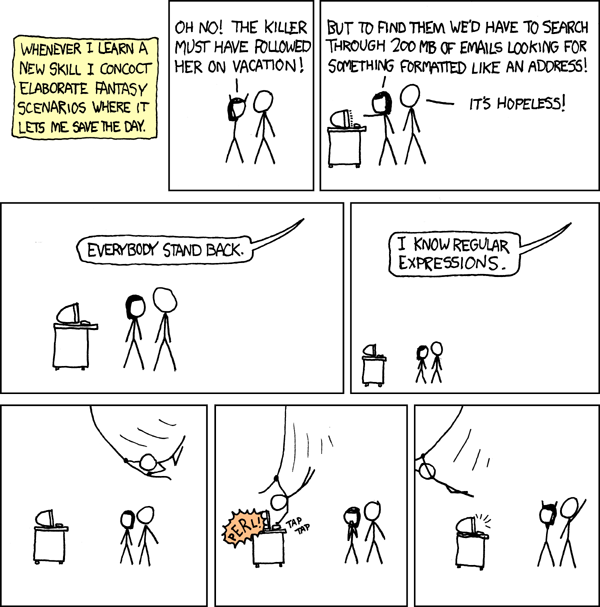
\includegraphics{images/xkcd}}
\end{center}
\end{frame}

\begin{frame}
  \frametitle{Eks. HTML formularer}
  HTML formularer indeholder input-felter, hvor
  brugeren kan indtaste tekststrenge.

  \begin{columns}
    \begin{column}{0.5\textwidth}
      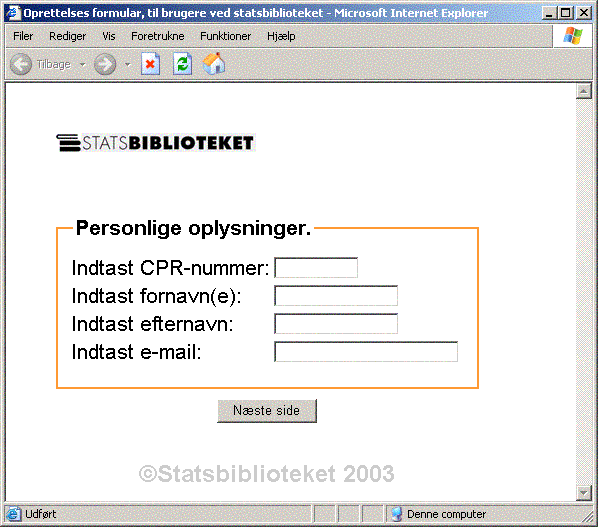
\includegraphics[width=\textwidth]{images/biblio}
    \end{column}

    \begin{column}{0.5\textwidth}
      For eksempel
      \begin{itemize}
      \item datoer
      \item telefonnumre
      \item CPR-numre
      \item emailadresser
      \item URL’er
      \item ...
      \end{itemize}
    \end{column}
\end{columns}

\end{frame}

\begin{frame}
\frametitle{HTML input valdidering}
\begin{itemize}[<+->]
\item Brugeren må ikke indtaste ugyldige strenge

\item Den traditionelle løsning: Programmer input validering i
JavaScript (til browseren – så input valideres løbende mens formularen udfyldes), og
Java (til serveren – for det tilfælde at browseren ikke udfører JavaScript-koden)
\item Problemer:
\begin{itemize}
\item Det er svært at programmere JavaScript, der virker på alle (nyere) browsere 
\item Vi skal skrive den samme kode i to forskellige sprog 
\item Store dele af koden skal skrives igen og igen...     
\end{itemize}
\end{itemize}
\end{frame}

\begin{frame}
\frametitle{Den datalogiske løsning}
\begin{itemize}[<+->]
\item Analysér problemområdet
\item Design et domæne-specifikt højniveau sprog
\item Lav en oversætter, der genererer JavaScript- og Java-koden fra højniveau specifikationer
\end{itemize}

Sproget \emph{PowerForms} er udviklet efter denne metode

Input-felter beskrives med \emph{regulære udtryk}, der oversættes til \emph{endelige automater}
\end{frame}

\section{Regulære udtryk}
\begin{frame}
\frametitle{Grundliggende begreber}
Vi starter med nogle \emph{matematiske definitioner}
\begin{itemize}[<+->]
\item Et \emph{alfabet} er en endelig mængde af tegn
\begin{itemize}
    \item Ex. $\{a,b,c,...z\}$
    \item Ex. ASCII, Unicode
    \item Ex. $\{0, 1\}$
\end{itemize}
\item En \emph{streng} er en \emph{endelig} sekvens af tegn fra alfabetet
\begin{itemize}
    \item Ex. \texttt{"onkel sune drejer den usle kno"}
    \item Ex. \texttt{"10110"}
    \item Ex. \texttt{"\,"}  (Den tomme streng. Skrives også $\Lambda$ (andre steder $\varepsilon$)).
\end{itemize}
\item Et \emph{sprog} er en mængde af strenge
\begin{itemize}
\item Ex. \texttt{\{"hans", "ole"\}}
\item Ex. $\{\Lambda, a, aa, aaa, aaaa, ...\}$
\item Ex. $\{\}$ (Det tomme sprog)
\item Ex. Alle korrekte danske sætninger
\end{itemize}
\end{itemize}
\end{frame}

\begin{frame}
\frametitle{Regulære udtryk}
Et \emph{regulært udtryk} beskriver et \emph{sprog}
\begin{itemize}
\item Regulære udtryk findes på 6 former
\item \textbf{3 basis-tilfælde:}
\begin{itemize}
\item $\emptyset$  	– den tomme mængde af strenge
\item $\Lambda$  	– mængden bestående af den tomme streng
\item $a\in\Sigma$	– mængden bestående af en enkelt streng, som
        	   er det ene tegn $a$ fra alfabetet $\Sigma$    
\end{itemize}
\item \textbf{Og 3 Sammensatte tilfælde (rekursive tilfælde):}
\begin{itemize}
\item $r_1+r_2$	– de strenge der beskrives af $r_1$ eller $r_2$
\item $r_1\dot r_2$	– de strenge der kan opdeles i to dele, så 
 	   venstre del beskrives af $r_1$ og højre del af $r_2$
\item $r^*$	– de strenge der kan opdeles i et antal dele,
		   der hver beskrives af $r$
    
\end{itemize}
\end{itemize}
\end{frame}

\begin{frame}
\frametitle{Eksempler på regulære udtryk}
\begin{itemize}[<+->]
\item Strenge over alfabetet $\{0,1\}$ med et \emph{lige} antal tegn:

$(00+11+01+10)^{*}$ eller $((0+1)(0+1))^{*}$
\item Strenge over alfabetet $\{0,1\}$ med et \emph{ulige} antal 1'er:

$0^{*}1(0^{*}10^{*}1)^{*}0^{*}$ eller $0^{*}10^{*}(10^{*}10^{*})^{*}$
\item Gyldige datoer, telefonnumre, CPR-numre, emailadresser, URL'er, \ldots
\end{itemize}
\end{frame}

\begin{frame}
\frametitle{Et mere realistisk eksempel}
Floating point tal i Pascal
\begin{itemize}[<+->]
\item Eksempler på gyldige strenge:  \texttt{``\f{3.14}''} \texttt{``\f{5.6E13}''} \texttt{``\f{-42.0}''}
\item $\Sigma = \{\f 0,\f 1,\f 2,\f 3,\f 4,\f 5,\f 6,\f 7,\f 8,\f 9,\f .,\f +,\f -,\f E\}$
\item Forkortelser:
\begin{itemize}
    \item $d=\f 0+\f 1+\f 2+\f 3+\f 4+\f 5+\f 6+\f 7+\f 8+\f 9$
    \item $r^{+} = r r^{*}$ (mindst én af r)
    \item $s = \Lambda + \f + + \f -$
\end{itemize}
\item Samlet udtryk: $sd^{+}(\f . d^{+} + \f . d^{+}\f E sd^{+} + \f E sd^{+} + \Lambda)$
\end{itemize}
\end{frame}

\begin{frame}
\frametitle{Genkendelse af strenge}
Givet en streng $x$, og et regulært udtryk $r$, hvordan ved vi om $r$ matcher $x$
% TODO: example
\begin{itemize}[<+->]
\item Den naive metode: vi prøver os frem:
\begin{itemize}
\item $\emptyset$ matcher intet
\item $\Lambda$ matcher kun den tomme streng.
\item $a\in\Sigma$ matcher kun  strengen bestående af den ene karakter \f a
\item $r_1 + r_2$ matcher hvis $r_1$ mathcer, eller $r_2$ matcher
\item $r_1 \cdot r_2$ Opdel $x$ så $x=x_1\cdot x_2$ på alle mulige måder
Og prøv om $r_1$ matcher $x_1$ og $r_2$ matcher $x_2$
\item $r_1^{*}$ Opdel $x$ så $x=x_1\cdot x_2\cdot\ldots\cdot x_n$ på alle mulige måder. Og se om
$r_1$ matcher alle $x_i$ for alle $i=1,\ldots, n$
\end{itemize}
\item Det virker! Men det er håbløst ineffektivt.
\end{itemize}
\end{frame}

\begin{frame}
  \begin{columns}
    \begin{column}{0.5\textwidth}
      \includegraphics[width=\textwidth]{images/1_seminar_even_num_zeroes}    
    \end{column}    
    \begin{column}{0.5\textwidth}
      \includegraphics[width=\textwidth]{images/1_seminar_pacman}
    \end{column}    
  \end{columns}

\frametitle{Endelige Automater (forsmag)}
\begin{itemize}
\item En endelig automat der genkender strenge over alfabetet $Σ = \{0,1\}$ med et \emph{lige} antal $0$'er
\item Automaten starter i den tilstand der er markeret med pilen
\item Den ``spiser'' et tegn af gangen af strengen fra venstre mod højre
\item Hvis den ender i tilstanden med dobbelt-cirkel, så accepterer den
%\item ... ellers ikke
\end{itemize}
\end{frame}

\begin{frame}
\frametitle{Kleenes sætning}
“Regulære udtryk og endelige automater 
 har samme udtrykskraft”
\begin{itemize}
\item \emph{Konstruktivt} bevis:
\item For ethvert regulært udtryk findes en ækvivalent endelig automat
\item For enhver endelig automat findes et ækvivalent regulært udtryk
\end{itemize}
\end{frame}

\begin{frame}
\frametitle{Powerforms eksempel}
\begin{itemize}
\item Lad $R$ være et regulært udtryk, der svarer til gyldige datoer på form \texttt{dd/mm-åååå}
\item Oversæt $R$ til en ækvivalent endelig automat $F$
\item Repræsenter $F$ som et JavaScript-program, der kan svare på om en streng $x$ er:
\begin{itemize}
\item \textbf{accepteret}
\item \textbf{ikke accepteret}, men der er en sti til accept
\item \textbf{ikke accepteret} og ingen sti til accept
\end{itemize}
\end{itemize}
\small\textbf{\url{http://www.brics.dk/bigwig/powerforms/examples/date.html}}
\end{frame}

\begin{frame}
\frametitle{Endelige automater til modellering af systemer}
\begin{itemize}
\item Endelige automater er også nyttige uden regulære udtryk
\item Endelige automater kan modellere systemer og egenskaber
\item De teoretiske resultater om endelige automater kan bruges til at kombinere modeller og verificere om et givet system har en given egenskab
\end{itemize}
\end{frame}

\begin{frame}
  \frametitle{En endelig automat, der modellerer en togsimulator (fra VisualSTATE)}
\begin{columns}
    \begin{column}{0.4\textwidth}
\begin{itemize}
\item 1421 del-automater
\item 11102 transitioner
\item 2981 inputs
\item 2667 outputs
\item 3204 lokale tilstande
\item Antal tilstande ialt: $10^{476}$
\end{itemize}        
    \end{column}
    \begin{column}{0.5\textwidth}
        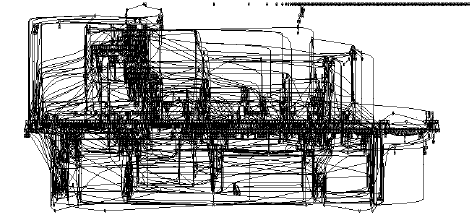
\includegraphics[width=1\textwidth]{images/1_seminar_futtog}
    \end{column}
\end{columns}
\begin{center}
Virker toget?
\end{center}
\end{frame}

\begin{frame}
\frametitle{Beregnelighed}
% TODO Make that figure
\begin{itemize}
\item Input og Output er strenge
\item Program er en algoritme som kører på en maskine
\item Eksempel: Givet et naturligt tal $N$ i binær repræsentation som Input,
beregn $N^2$ som output.
\end{itemize}
\end{frame}

\begin{frame}
\frametitle{Beslutningsproblemer}
% TODO Make that figure
\begin{itemize}
\item Hvis vi ignorerer effektivitet, så kan alle beregningsproblemer omformuleres til beslutningsproblemer.
\item Eksempel: Givet to naturlige tal $N,M$ i binær repræsentation som Input,
svar ja hvis og kun hvis $N^2 = M$
\end{itemize}
\end{frame}

\begin{frame}
\frametitle{Beslutningsproblemer som sprog}
\begin{itemize}[<+->]
\item Ethvert beslutningsproblem er et sprog (en mængde af strenge)
\item $L = \{ x | P(X) = \text{ja} \}$
\item Ethvert sprog $L$ er også et beslutningsproblem: 
\[P(x) = 
\begin{cases}
ja & \text{hvis } x ∈ L \\
nej & \text{ellers }
\end{cases}
\]
\end{itemize}
\end{frame}

\begin{frame}
\frametitle{Eksempler på beslutningsproblemer}
{\large Givet en streng $x$,}
\begin{itemize}
\item er den en gyldig dato på form dd/mm-åååå?
\item er den et syntaktisk korrekt Java program?
\item er den et primtal?
\item er den en konfiguration i skak hvor det er muligt for hvid at
  vinde?
\item er den et semantisk korrekt Java-program?
\item er den en syntaktisk korrekt sætning i dansk?
\item er den en litterær klassiker?
\item — vi vil kun se på formelle sprog og veldefinerede problemer
\end{itemize}
\end{frame}

\begin{frame}
\frametitle{Endelige automater som model for beregnelighed}
Vi vil studere følgende emne:
\begin{itemize}
\item Hvilke problemer kan afgøres af en maskine 
med endeligt meget hukommelse?
\item Med andre ord:
Hvilke sprog kan genkendes af 
endelige automater?
\end{itemize}
\end{frame}

\begin{frame}
\frametitle{Mere generelle modeller for beregnelighed}
\begin{itemize}
\item Pushdown-automater:
\begin{itemize}
\item endelige automater med adgang til en vilkårligt stor stak (last-in-first-out)
\item anvendes ofte i parsere i oversættere
\item svarer til kontekstfri grammatikker
\end{itemize}
\item Turing-maskiner:
\begin{itemize}
\item ligesom endelige automater med adgang til en uendeligt stor notesblok
\item kan udføre vilkårlige algoritmer (Church-Turing-tesen)
\item svarer til uindskrænkede grammatikker (hvor endelige automater svarer til regulære grammatikker)
\end{itemize}

\end{itemize}
\end{frame}

\begin{frame}
\frametitle{Klasser af formelle sprog}
\begin{center}
    \includegraphics[width=1\textwidth]{images/1_seminar_fried_egg}
\end{center}
\pause
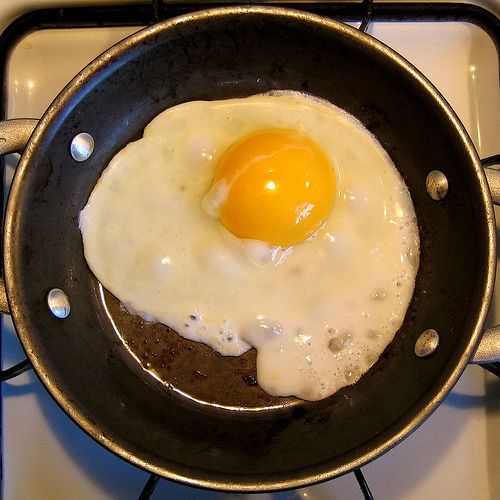
\includegraphics[width=.2\textwidth]{images/1_seminar_real_egg}\\
{\tiny Picture from \url{http://www.flickr.com/photos/33602849@N00/5894257}}
\end{frame}

\begin{frame}
\frametitle{Hvorfor så nøjes med regulære automater}
\begin{itemize}
\item Klassen af regulære sprog har mange “pæne” egenskaber:
\begin{itemize}
\item afgørlighed (f.eks, “givet en FA M, accepterer den nogen strenge overhovedet?”)
\item lukkethed (snit, forening, ...)
\end{itemize}

\item Til sammenligning:

\begin{itemize}
\item Ved Turing-maskiner er næsten alt uafgørligt
(Rices sætning: “alt interessant vedrørende sproget for en Turing-maskine er uafgørligt”)
\item Pushdown-automater / kontekstfri grammatikker:
en mellemting, både med hensyn til udtrykskraft og afgørlighedsegenskaber
\end{itemize}

\end{itemize}
\end{frame}

\begin{frame}
\frametitle{Uafgørlighed}
\begin{center}
\fbox{
\parbox{3cm}{
while (x≠1) \{

\hspace{0.5cm} if (even(x))

\hspace{1cm} x = x/2;

\hspace{0.5cm} else

\hspace{1cm} x = 3·x+1;

\}
}
}
\end{center}
\begin{itemize}
\item Terminerer dette program på alle input $x$? Ja eller nej?
\item Tilsyneladende ja, men ingen har endnu bevist det!
\item Men vi kan bevise, at der ikke findes et program (=en Turing-maskine), 
der kan afgøre det generelle problem “givet et program P, terminerer P på alle input?”
\end{itemize}

\end{frame}

\begin{frame}
\frametitle{Praktiske oplysninger om kurset}
\begin{itemize}
\item Hjemmeside: \url{http://cs.au.dk/~stm/RegAut}
\item Seminarer: % TODO: Find dates:
\begin{itemize}
\item XXX (i dag)
\item XXX
\item XXX
\end{itemize}

\end{itemize}
\end{frame}

\begin{frame}
\frametitle{Materiale}
\begin{itemize}
\item 
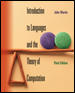
\includegraphics[width=0.2\textwidth]{images/1_seminar_bog}\\
John Martin
Introduction to Languages and 
the Theory of Computation
3. udgave, McGraw-Hill, 2002
ISBN: 0071198547 eller 0072322004
\item Opgaver på ugesedlerne
\end{itemize}
\end{frame}

\begin{frame}
\frametitle{Aktivitetsniveau}
\begin{itemize}
\item Forventet aktivitet per uge \url{~} 15 timer
\item 6 uger · 15 timer/uge = 90 timer
\item Seminarer: 21 timer
\item Mellem seminarer: 69
\item Forventet hjemmearbejde ca. 11 timer per uge
\item Det forventes at man:
\begin{itemize}
\item Læser de relevante kapitler i bogen
\item Løser opgaverne
\item Laver programmeringsprojektet
\end{itemize}
\end{itemize}
\end{frame}

\begin{frame}
\frametitle{Opgaver}
\begin{itemize}
\item Teoretiske opgaver
\begin{itemize}
\item udfordrer forståelsen af det 
gennemgåede materiale
øvelse i typisk “datalogisk matematik”
\end{itemize}
\item Programmeringsprojekt 
\begin{itemize}
\item (dRegAut Java-pakken)
implementation af de gennemgåede algoritmer, der udledes af konstruktive beviser
Øvelse i at implementere formelle specifikationer i Java.
\end{itemize}
\end{itemize}
\end{frame}

\begin{frame}
\frametitle{Eksamen}
\begin{itemize}
\item Mundtlig, ekstern censur, 13-skalaen
20 min. per person, uden forberedelsestid 
\item For at kunne indstilles til eksamen skal man have godkendt besvarelser af de obligatoriske opgaver
\end{itemize}
\end{frame}

\begin{frame}
\frametitle{Alfabeter, strenge og sprog}
\begin{itemize}
\item 
Et alfabet $Σ$ er en endelig mængde (af tegn/symboler)
eks.:  $Σ={a,b,c}$
\item
En streng x er en endelig sekvens af tegn fra alfabetet
eks.:  $x=abba$
$Λ$ repræsenterer den tomme streng (strengen af længde 0), $Λ∉Σ$
\item
Et sprog $L$ er en (vilkårlig) mængde af strenge
eks.:  $L={Λ,cab,abba}$
\item
$Σ^*$ er mængden af alle strenge over $Σ$
dvs. $L⊆Σ^*$ hvis $L$ er et sprog over $Σ$
eks.:  hvis $Σ={a,b,c}$ så er $Σ^*={Λ,a,b,c,aa,ab,ac,aaa,aab,...}$
\end{itemize}
\end{frame}

\begin{frame}
\frametitle{Konkatenering af strenge}
\begin{itemize}
\item Hvis $x,y∈Σ^*$, så er $x·y$ (konkateneringen af $x$ og $y$) den streng, der fremkommer ved at sætte tegnene i $x$ før tegnene i $y$
\begin{itemize}
\item Eks.:  hvis  $x=abb$  og  $y=a$, så er 
\[x·y=abba\]
\[y·x=aabb\]

\end{itemize}

\item Bemærk:  $x·Λ=Λ·x=x$  for alle x
\item $x·y$ skrives ofte xy (uden “·”)
\end{itemize}
\end{frame}

\begin{frame}
\frametitle{Konkatenering af sprog}
\begin{itemize}
\item Hvis $L_1,L_2⊆Σ^*$, så er $L_1·L_2$  (konkateneringen af 
$L_1$ og $L_2$) defineret ved
	 \[L_1·L_2 = \{x·y | x∈L_1 ∧ y∈L_2\}\]

\item Eks.: Hvis $Σ=\{0,1,2,a,b,c\}$ og
$L_1=\{Λ,10,212\}$, 
$L_2=\{cab,abba\}$ så er: 
\[L1·L2 =\{cab,10cab,212cab,abba,10abba,212abba\}\]
\item Bemærk:
\begin{itemize}
\item $L·\{Λ\} = \{Λ\}·L = L$  for alle $L$
\item $L·∅ = ∅·L = ∅$  for alle $L$
\item $L_1·L_2$ skrives ofte $L_1L_2$ (uden “$·$”)
\end{itemize}
\end{itemize}
\end{frame}

\begin{frame}
\frametitle{Kleene stjerne}
Kleene stjerne er en måde at udtrykke ``0 eller flere forekomster''
\begin{itemize}
\item $L^k = \explain{LL···L}{\text{$k$ gange}}$
	   (konkatenering af $k$ forekomster af $L$)
\item $L^0 = \{Λ\}$ (0 forekomster af $L$)
\item \textbf{$L^* = \bigcup_{i=0}^∞{L^i}$ (Kleene stjerne af L)}
\item $L^+ = L^*L$ (1 eller flere forekomster)
\item Eks.: Hvis $L=\{aa,b\}$ så er
\[L^*=\{Λ,aa,b,aaaa, aab, baa, bb, aaaaaa, … \}\]
\end{itemize}
\end{frame}

\begin{frame}
\frametitle{Rekursive definitioner}

\begin{itemize}
\item En definition er rekursiv, hvis den
refererer til sig selv

\item Eks.:   Fibonacci $f : N→N$
	\[f(n) = \begin{cases}
                     1,& \text{ hvis } n=1 ∨ n=0 \\
                     f(n-1)+f(n-2), & \text{ellers}
                 \end{cases} \]

\item Enhver selv-reference skal referere til noget ”mindre” og dermed
  føre til endeligt mange selv-referencer
\end{itemize}
\end{frame}

\begin{frame}
\frametitle{Rekursiv definition af strenge}
\begin{itemize}
\item $x$ er en streng over alfabetet $Σ$, dvs. $x∈Σ^*$ hvis:
\item $x=Λ$, eller
\item $x=y·a$ hvor $y∈Σ^*$ og $a∈Σ$
\item (underforstået $Σ^*$ er den mindste mænge der opfylder dette)
\item Eksempel:  
\[abc = (((Λ·a)·b)·c) ∈ Σ^*,   (\text{hvor } Σ=\{a,b,c,d\})\]
\end{itemize}
\end{frame}

\begin{frame}
\frametitle{Syntax af regulære udtryk}
Mængden $R$ af regulære udtryk over $Σ$ er 
den mindste mængde, der indeholder følgende:
\begin{itemize}
\item $∅$ 
\item $Λ$ 
\item $a$ for hver $a∈Σ$
\item $(r_1+r_2)$ hvor $r_1,r_2∈R$
\item $(r_1r_2)$  hvor $r_1,r_2∈R$
\item $(r^*)$  hvor $r∈R$
\end{itemize}
\end{frame}


\begin{frame}
\frametitle{Semantik af regulære udtryk}
Sproget $L(r)$ for $r∈R$ er defineret rekursivt i strukturen af $R$
\begin{itemize}
\item $L(∅) = ∅$ 
\item $L(Λ) = \{ Λ \}$ 
\item $L(a) = \{ a \}$
\item $L((r_1+r_2))= L(r_1)∪L(r_2)$ 
\item $L((r_1r_2))=L(r_1)L(r_2)$  
\item $L((r^*)) = (L(r))^*$
\end{itemize}
\end{frame}

\begin{frame}
\frametitle{Regulære sprog}
\begin{itemize}
\item Definition:
Et sprog $S$ er regulært hvis og kun hvis
der eksisterer et regulært udtryk $r$ hvor $L(r)=S$
\end{itemize}
\end{frame}

\begin{frame}
\frametitle{Paranteser i regulære udtryk}
\begin{itemize}[<+->]
\item Forening og konkatenering er \textbf{associative}, så vi vælger at tillade f.eks.
\begin{itemize}
\item at $(a+(b+c))$ kan skrives $a+b+c$
\item at $(a(bc))$ kan skrives $abc$
\end{itemize}
\item Vi definerer \textbf{præcedens} for operatorerne:
\begin{itemize}
\item ${}^*$ binder stærkest
\item konkatenering binder middel
\item $+$ binder svagest
\item Eks.:   $(a+((b^*)c))$ kan skrives $a+b^*c$
\end{itemize}
\end{itemize}
\end{frame}

\begin{frame}
\frametitle{Eksempel}
\begin{itemize}[<+->]
\item Betragt følgende regulære udtryk $r$ over alfabetet $\{0,1\}$:
\[r = (1+Λ)001\]
\item På grund af parentesreglerne er dette det samme som
\[r = ((((1+Λ)0)0)1)\]
\item Så sproget for $r$ er
\[L(r) = (((\{1\}∪\{Λ\})\{0\})\{0\})\{1\})
 = \{1001,001\}\]
\end{itemize}
\end{frame}

\begin{frame}
\frametitle{Quiz}
\begin{enumerate}
\item Hvad betyder $\{a,bc\}^*$?
\item Hvad er betingelsen for at et 
sprog $S$ er regulært?
\end{enumerate}
\end{frame}

\begin{frame}
\frametitle{Øvelser}
\begin{itemize}
\item{} [Martin] Opg. 3.2
\item{} [Martin] Opg. 3.9 (a-e)
\item{} [Martin] Opg. 3.10 (a-b)
\end{itemize}
\end{frame}

\section{Induktionsbevis}
\begin{frame}
\frametitle{Reverse-operatoren}
\begin{itemize}
\item Givet en streng $x∈Σ^*$, definer $reverse(x)$ rekursivt i strukturen af x:
\item $reverse(Λ) = Λ$
\item $reverse(ya) = a(reverse(y))$, hvor $y∈Σ*, a∈Σ$
\item Eksempel: $reverse(123) = 3·reverse(12) = … = 321·reverse(Λ)= 321$
\end{itemize}
\end{frame}

\begin{frame}
\frametitle{Reverse på et sprog}
\begin{itemize}
\item Givet et sprog L⊆Σ*, definer
\[reverse(L) = \{ reverse(x) | x∈L \}\]
\item Eksempel:
Hvis L=\{Λ,123,abc\} så er
\[reverse(L)=\{Λ,321,cba\}\]
\end{itemize}
\end{frame}

\begin{frame}
\frametitle{Rekursion og induktionsbeviser}
\begin{itemize}[<+->]
\item Rekursive definitioner giver ofte anledning til induktionsbeviser

\item Hvis vi skal bevise noget på form ``for alle $X$ gælder $P(X)$'', hvor
  mængden af $X$’er er defineret rekursivt, så kan vi prøve
  bevisteknikken ``induktion i strukturen af $X$''
\end{itemize}
\end{frame}

\begin{frame}
\frametitle{Eksempel på et induktionsbevis (1/3)}
\begin{itemize}[<+->]
\item Påstand:  Hvis $S$ er et regulært sprog, så er $reverse(S)$ også regulært  

(dvs. de regulære sprog er lukkede under Reverse)
\item Bevis: 

S er regulært, så der eksisterer et regulært udtryk $r$ så $L(r)=S$

Vi vil vise ved \textbf{induktion} i strukturen af $r$, at der eksisterer et
regulært udtryk $r’$ hvor $L(r’)=reverse(L(r))$, hvilket medfører, at
$reverse(S)$ er regulært
\end{itemize}
\end{frame}

\begin{frame}
\frametitle{Eksempel på et induktionsbevis (2/3)}
Basis
\begin{itemize}
\item $r = ∅$: $r' = ∅$
\[L(∅) = ∅ = reverse(∅) = reverse(L(∅))\]
\item $r = Λ$: $r' = Λ$
\[…\]
\item $r = a$: $r' = a$
\[…\]
\end{itemize}
\end{frame}

\begin{frame}
\frametitle{Eksempel på et induktionsbevis (3/3)}
Induktionsskridtet

For alle deludtryk $s$ af $r$ kan vi udnytte
\textbf{induktionshypotesen}:

Der eksisterer et regulært
udtryk $s’$ hvor $L(s’)=Reverse(L(s))$
\pause
\begin{itemize}[<+->]
\item \underline{$r = r₁+r₂$} hvor $r₁, r₂∈R$: vælg $r' = r₁' + r₂'$ hvor $r₁'$ of
  $r₂'$ er givet i induktionshypotesen.
\item \underline{$r = r₁r₂$} hvor $r₁, r₂∈R$: vælg $r' = r₂'r₁'$
\item \underline{$r = r₁^*$} hvor $r₁∈R$: vælg $r' = (r₁')^*$
\item \underline{Lemma 1:}
$∀x,y∈Σ^*$: $reverse(xy)=
         reverse(y)reverse(x)$

\textbf{Bevis:} induktion i strukturen
(eller længden) af $y$

\item \underline{Lemma 2:}
$∀i≥0,E⊆Σ^*$:
  $reverse(E^i) = (reverse(E))^i$

\textbf{Bevis}: induktion i $i$

\end{itemize}

\end{frame}

\begin{frame}
\frametitle{Konstruktive beviser}
\begin{itemize}
\item Bemærk at dette induktionsbevis implicit indeholder en algoritme
  til – givet et regulært udtryk for $S$ – at konstruere et regulært
  udtryk for $reverse(S)$

\item Sådanne beviser kaldes konstruktive

\item Husk altid både \emph{konstruktionen} \textbf{og} \emph{beviset for dens korrekthed}
\end{itemize}
\end{frame}

\begin{frame}
\frametitle{Algoritmen}
\begin{itemize}[<+->]
\item Input: et regulært udtryk $r$
\item Definer en rekursiv funktion REV ved:
\begin{itemize}
\item $REV(∅) = ∅$
\item $REV(Λ) = Λ$
\item $REV(a) = a$,  hvor $a∈Σ$
\item $REV(r_1+r_2) = REV(r_1) + REV(r_2)$
\item $REV(r_1r_2) = REV(r_2)·REV(r_1)$
\item $REV(r_1^*) = (REV(r_1))^*$
\end{itemize}
\item Output: det regulære udtryk $REV(r)$
\end{itemize}
\end{frame}

\begin{frame}
\frametitle{Øvelse}
\begin{itemize}
\item Lad $r$ være det regulære udtryk $((a+Λ)cbc)^*$ over alfabetet
  $\{a,b,c\}$. 
\begin{itemize}
\item   Bevis at enhver streng i sproget sproget $L(r)$ har et
  lige antal $c$'er. 
\item   Argumentér kort og præcist for hvert trin i
  beviset.
\end{itemize}

\item Hint: Brug definitionen af sprog for regulære udtryk (Definition
  3.1 i [Martin] ), definitionen af ${}^*$ på sprog (s. 31 øverst i
  [Martin]), og lav induktion.
\end{itemize}
\end{frame}

% TODO Why is this slide here???
% \begin{frame}
% \frametitle{dRegExp}
% \begin{itemize}
% \item Java-repræsentation af regulære udtryk

% \item Speciel syntax:
% \begin{itemize}
% \item \# betyder $∅$
% \item \% betyder $Λ$
% \end{itemize}
% \item Alfabetet angives som en mængde af Unicode tegn
% \end{itemize}
% \item Eks.: $((a+Λ)cbc)^*$ skrives som ``((a+\%))cbc)*''
% \end{frame}
 
\begin{frame}
\frametitle{Løsninger}
\begin{itemize}[<+->]
\item [] [Martin] 3.2
\begin{itemize}
\item a) 00 
\item b) 01 
\item c) 0 
\item d) 010
\end{itemize}
\end{itemize}
\end{frame}

\begin{frame}
\frametitle{Løsninger}
\begin{itemize}
% TODO check these when you find the book
\item a) $1^*01^*01^*$
\item b) $(0+1)^*0(0+1)^*0(0+1)^*$
\item c) $+ 1 + (0+1)^*0 + (0+1)^*11$
\item d) $(00 + 11)(0+1)^* + (0+1)^*(00 + 11)$
\item e) $(1 + 01)^*(0 + )$ 

\end{itemize}
\end{frame}
\section{Regulære automater}

\begin{frame}
\frametitle{Regulære udtryk vs endelige automater}
\begin{itemize}
\item  Regulære udtryk: deklarative
\begin{itemize}
\item dvs. ofte velegnede til at specificere regulære sprog
\end{itemize}
\item Endelige automater: operationelle
\begin{itemize}
\item dvs. bedre egnet til at afgøre om en given streng er i sproget
\end{itemize}
\item Ethvert regulært udtryk kan oversættes til en
endelig automat – og omvendt
\begin{itemize}
\item (bevises næste seminar...)
\end{itemize}
\end{itemize}
\end{frame}

\begin{frame}
\frametitle{En endelig automat}
\begin{itemize}
\item   En endelig automat, der genkender strenge over alfabetet
$Σ=\{0,1\}$ med ulige antal 1’er:

\begin{center}
  \includegraphics[width=0.3\textwidth]{images/1_seminar_odd_num_ones}
\end{center}
\item Automaten læser strengen ét tegn ad gangen,
fra venstre mod højre
\item Hvis automaten ender i en accept-tilstand, så
accepteres(=genkendes) strengen
\end{itemize}
\end{frame}

\begin{frame}
  \frametitle{At køre en streng på en automat}
\begin{itemize}
\item Eksempel: vi vil vide om strengen $1010$ accepteres
\begin{center}
  \includegraphics[width=0.3\textwidth]{images/1_seminar_odd_num_ones}
\end{center}
\item Vi starter i starttilstanden og læser strengen ét tegn ad gangen
\item Vi ender i en ikke-accept tilstand, så strengen accepteres ikke
\end{itemize}
\end{frame}

\begin{frame}
  \frametitle{Hvad repræsenterer tilstandende}
  \begin{itemize}
  \item  Hver tilstand repræsenterer en viden om den hidtil
læste delstreng
\item Eksempel:
\begin{center}
  \includegraphics[width=0.3\textwidth]{images/1_seminar_odd_num_ones}
\end{center}
\item X: “der er læst et lige antal 1’er”
\item Y: “der er læst et ulige antal 1’er”

  \end{itemize}
\end{frame}

\begin{frame}
\frametitle{Formel definition af endelige automater}
\begin{itemize}
\item  En endelig automat (finite automaton/FA) er
et 5-tupel $(Q, Σ, q_0, A, δ)$ hvor
\item $Q$ er en endelig mængde af tilstande
\item $Σ$ er et alfabet
\item $q_0∈Q$ er en starttilstand
\item $A⊆Q$ er accepttilstandene
\item $δ: Q×Σ→Q$ er en transitionsfunktion
\end{itemize}
\end{frame}

\begin{frame}
  \frametitle{Eksempel}
  \begin{itemize}
  \item  Denne grafiske repræsentation af en automat:
\begin{center}
  \includegraphics[width=0.3\textwidth]{images/1_seminar_odd_num_ones}
\end{center}
  \item svarer til 5-tuplet $(Q, Σ, q_0, A, δ)$ hvor
 \item $Q = \{X,Y\}$
 \item $Σ = \{0,1\}$
 \item $q_0 = X$
 \item $A = \{Y\}$
 \item $δ: Q×Σ→Q$ er denne funktion:

\begin{center}
  \begin{tabular}{c|c c}
    & 0 & 1 \\
    \hline
    X& X& Y \\
    Y& Y & X \\
  \end{tabular}
\end{center}
  \end{itemize}
\end{frame}

\begin{frame}
  \frametitle{Hvorfor en formel definition}
  \begin{itemize}
  \item   Den formelle definition viser kort og præcist
hvad en FA er
\item For eksempel,
\begin{itemize}[<+->]
\item en FA har endeligt mange tilstande
\item den har præcis én starttilstand
\item en vilkårlig delmængde af tilstandene kan være
accepttilstande
\item for enhver tilstand $q$ og alfabetsymbol $a$ er der én
udgående transition (til tilstanden $δ(q,a)$)
\item der er ikke noget krav om, at alle tilstande kan nås
fra starttilstanden
\end{itemize}
  \end{itemize}
\end{frame}

\begin{frame}
  \frametitle{Sproget af en automat}
\begin{itemize}
\item 5-tupel-definitionen fortæller hvad en FA er
\item Vi vil nu definere hvad en FA kan:
\item En FA accepterer en streng, hvis dens kørsel fra
starttilstanden ender i en accepttilstand
\item Sproget $L(M)$ af en FA $M$ er mængden af strenge, den
accepterer
\item $M$ genkender sproget $L(M)$
  \end{itemize}
\end{frame}

\begin{frame}
  \frametitle{Formel definition af L(M)}
  \begin{itemize}[<+->]
  \item  Givet en FA $M=(Q, Σ, q_0, A, δ)$, definer
den udvidede transitionsfunktion $δ^*: Q×Σ^*→Q$
ved
\[δ^*(q, x) = \begin{cases}
 q &\text{ hvis }x=Λ\\
 δ(δ^*(q, y), a)  & \text{ hvis } x=ya \text{ hvor } y∈Σ^*\text{ og } a∈Σ
\end{cases}
\]
\item $x∈Σ^*$ accepteres af $M$ hvis og kun hvis $δ^*(q_0, x)∈A$
\item Definer $L(M) = \{ x ∈ Σ^* | x\text{ accepteres af }M \}$
  \end{itemize}
\end{frame}

\begin{frame}
  \frametitle{Quiz}
Konstruer en FA så

\begin{tabular}{lc}
 $L(M) = Σ^*$ &
\visible<2->{\imagetop{\includegraphics[scale=0.2]{images/1_seminar_everything}}}\\
$L(M) = ∅$ &
\visible<3->{\imagetop{\includegraphics[scale=0.2]{images/1_seminar_nothing}}} \\
 $L(M) = \{a\}$ &
\visible<4->{\imagetop{\includegraphics[scale=0.2]{images/1_seminar_only_a}}} \\
 $L(M) = \{ x∈Σ^* | n_a(x)\text{ lige og } n_b(x) \text{ ulige}\}$ &
\visible<5->{\imagetop{\includegraphics[scale=0.2]{images/1_seminar_even_a_odd_b}}} \\
\end{tabular}

\end{frame}

\begin{frame}
  \frametitle{Øvelser}
\begin{itemize}
\item{} [Martin] Opg. 3.17 (e)
\item{} [Martin] Opg. 3.18
\item{} [Martin] Opg. 3.19 (a-c)
\end{itemize}
\end{frame}

\section{Skelnelighed og produktkonstruktion}

\begin{frame}
  \frametitle{Skelnelighed}
  \begin{itemize}
  \item   Givet et sprog $L$, hvor mange tilstande er
nødvendige \\ i en FA $M$ hvis $L(M)=L$?
\item To strenge, $x$ og $y$, skal ende i forskellige
tilstande,\\ hvis der er behov for at kunne
\textbf{skelne} dem:
\item dvs., $δ^*(q_0, x) ≠ δ^*(q_0, y)$
      hvis $∃z∈ Σ^*: (xz∈L ∧ yz∉L) ∨ 
                  (xz∉L ∧ yz∈L)$

  \end{itemize}
\end{frame}

\begin{frame}
  \frametitle{Definition af skelnelighed}
  \begin{itemize}
  \item Lad $L⊆Σ^*$ og $x,y∈Σ^*$
\item 
\textbf{Kvotientsproget} $L/x$ defineres som
   \[ L/x = \{ z∈ Σ^* | xz∈L \}\]
\item $x$ og $y$ \textbf{er skelnelige} mht. $L$ hvis
\[L/x ≠ L/y\]
\item $z$ \textbf{skelner} $x$ og $y$ mht. $L$ hvis
\[z∈L/x - L/y\text{ eller }z∈L/y - L/x\]

  \end{itemize}
\end{frame}

\begin{frame}
  \frametitle{Eksempel}
  \begin{itemize}
  \item Hvis
\begin{itemize}
\item $L = \{ s∈\{0,1\}^* | s\text{ ender med }10 \}$
\item $x = 00$
\item $y = 01$
\end{itemize}
    \item så er $x$ og $y$ skelnelige mht. $L$
\item Bevis:
   $z = 0$ skelner $x$ og $y$
\item Heraf kan vi se, at hvis $M=(Q, Σ, q_0, A, δ)$ genkender $L$
  så er \[δ^*(q_0, x) ≠ δ^*(q_0, y)\]
Uanset hvordan $M$ ellers er opbygget.
  \end{itemize}
\end{frame}

\begin{frame}
  \frametitle{Nødvendigt antal tilstande i en FA}
  \begin{itemize}
  \item Antag $x_1, x_2, …, x_n∈ Σ^*$ \\
    og for ethvert par $x_i,x_j, i≠j$
    er $x_i$ og $x_j$ skelnelige mht. $L$
  \item Enhver FA der genkender $L$ har mindst
    $n$ tilstande
  \item Bevis (skitse):
\begin{itemize}[<+->]
\item Antag FA'en har færre tilstande
\item Det medfører at $∃i≠j: δ^*(q₀,x_i)=δ^*(q₀,x_j)$ (skuffeprincippet)
\item Det er i modstrid med at $x_i$ og $x_j$ var skelnelige mht. $L$
\end{itemize}
  \end{itemize}
\visible<2->{
\begin{center}
  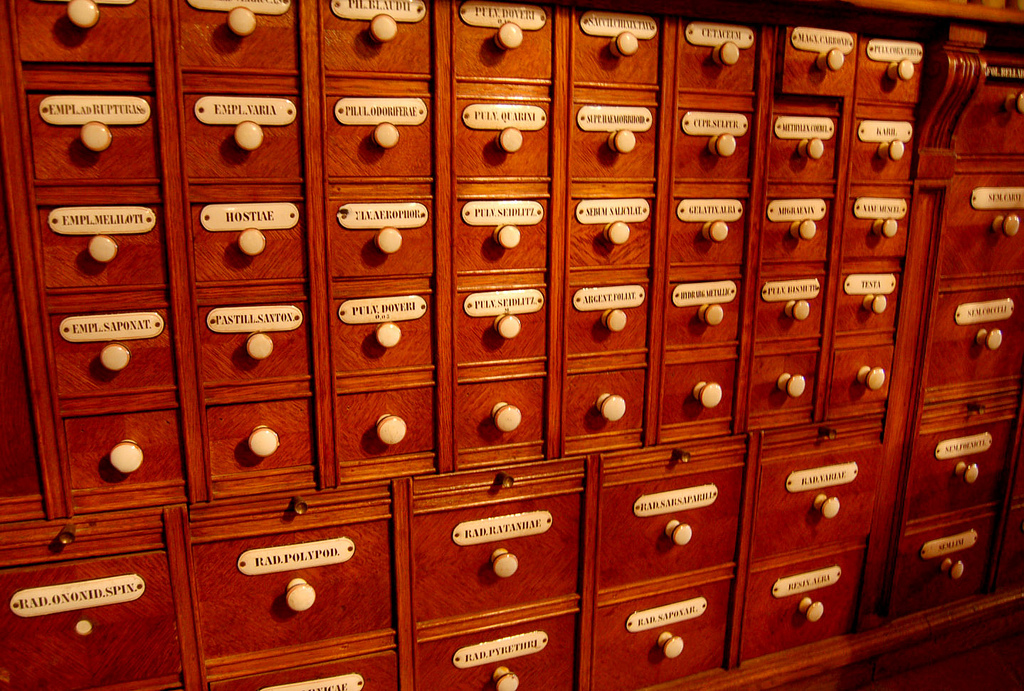
\includegraphics[width=0.25\textwidth]{images/1_seminar_skuffe}\\
  {\tiny \url{http://www.flickr.com/photos/curiousexpeditions/2194711073/}}
\end{center}}
\end{frame}


\begin{frame}
  \frametitle{Eksempel 1: En stor automat}
  \begin{itemize}[<+->]
\item Dette eksempel kan give intuition for begrebet skelnelighed
  \item Lad $L_{42} = \{ x∈\{0,1\}^* | |x|≥42\text{ og det 42. symbol
                           fra højre i $x$ er et }1 \}$
\item Lad $x_1, x_2, ..., x_{2^{42}}$ være alle strenge af længde 42
over alfabetet $\{0,1\}$
\item Disse strenge er alle parvist skelnelige mht. $L_{42}$
\item En automat der genkender $L_{42}$ har derfor
mindst $2^{42}$ tilstande
\item (...hvis den overhovedet findes)
\item Bevis: $x≠y$ må være forskellige i $i$'te tegn fra venstre.
  Strengen $z$ som skelner kan være $0^{i-1}$
\end{itemize}
\end{frame}

\begin{frame}
  \frametitle{Eksempel 2: Palindromer}
  \begin{itemize}[<+->]
  \item Lad $pal = \{ x∈\{0,1\}^* | x=reverse(x) \}$
\item Lad $x$ og $y$ være vilkårlige forskellige
strenge over $\{0,1\}$
\item $x$ og $y$ er skelnelige mht. $pal$ (bevis: se bogen...) % TODO Find chapter
\item Vi kan altså finde en vilkårligt stor mængde parvist skelnelige
  strenge, så $pal$ er ikke regulært.

  \end{itemize}
\end{frame}

\begin{frame}
  \frametitle{Forening af regulære sprog}
  \begin{itemize}
  \item  Givet to regulære sprog, $L_1$ og $L_2$
er $L_1 ∪ L_2$ også regulært?
\item Ja!  (dvs. klassen af regulære sprog er lukket under forening)
  \end{itemize}
\end{frame}

\begin{frame}
  \frametitle{Eksempel}
\begin{tabular}{lc}
  M1:
(strenge med lige antal 0’er) & 
\imagetop{\includegraphics[scale=.25]{images/1_seminar_even_num_zeroes_label}}
\\
M2:     
  (strenge der ender med 0) & 
\imagetop{\includegraphics[scale=.25]{images/1_seminar_ends_with_zero}}
\\
  L(M) = L(M1) ∪ L(M2) & 
\imagetop{\includegraphics[scale=.25]{images/1_seminar_union}}
\end{tabular}  
\end{frame}

} % ignore


\begin{frame}
  \frametitle{Produktkonstruktionen}
  \begin{itemize}
  \item Antag vi har to FA’er:
\item $M_1 = (Q_1, Σ, q_1, A_1, δ_1)$
\item $M_2 = (Q_2, Σ, q_2, A_2, δ_2)$
\item Definer en ny FA: $M = (Q, Σ, q_0, A, δ)$ hvor
\begin{itemize}
\item $Q = Q_1×Q_2$ (produktmængden af tilstande)
\item $q_0 = (q_1, q_2)$
\item $A = \{ (p, q) | p∈A_1 ∨ q∈A_2 \}$
\item $δ((p, q), a) = (δ_1(p, a), δ_2(q, a))$
\end{itemize}
\item Der gælder nu:
\[L(M) = L(M_1) ∪ L(M_2)\]
  \end{itemize}
\end{frame}

\begin{frame}
  \frametitle{Konstruktivt bevis for korrekthed}
  \begin{itemize}
  \item  Lemma:
  $∀x∈Σ^*: δ^*((p, q), x) = (δ_1^*(p, x), δ_2^*(q, x))$
\item   (Bevis: opgave 3.32, induktion i $x$) \\
\begin{itemize}
\item Brug lemmaet samt definitionerne af $M$ og $L(\bullet)$
\end{itemize}


  \end{itemize}
\end{frame}

\begin{frame}
  \frametitle{Nøjes med opnåelige tilstande}
  \begin{itemize}
  \item          Nøjes med opnåelige tilstande
\item Produktkonstruktionen bruger $Q = Q_1×Q_2$
\item I praksis er hele tilstandsrummet sjældent nødvendigt
\item Eksempel:
  \imagetop{
\includegraphics[scale=.25]{images/1_seminar_even_num_zeroes_label}}
\ \ \imagetop{
\includegraphics[scale=.25]{images/1_seminar_even_num_zeroes_label2}}\\
  \includegraphics[scale=.25]{images/1_seminar_union2}
\item Kun tilstande, der er opnåelige fra starttilstanden er
relevante for sproget!

  \end{itemize}
\end{frame}

\begin{frame}
  \frametitle{Snitmængde og differens}
  \begin{itemize}
\item Givet to regulære sprog, $L_1$ og $L_2$
\begin{itemize}
\item  er $L_1∩L_2$ også regulært?
\item  er $L_1-L_2$ også regulært?
\end{itemize}
\pause
\item Ja! (dvs. klassen af regulære sprog er lukket under snit og differens)
\item Bevis: produktkonstruktion som ved ∪ men
\begin{itemize}
\item for $∩$, vælg $A = { (p, q) | p∈A_1 ∧ q∈A_2 }$
\item for $-$, vælg $A = { (p, q) | p∈A_1 ∧ q∉A_2 }$
\end{itemize}
\end{itemize}
\end{frame}


\begin{frame}
  \frametitle{Komplement}
  \begin{itemize}
  \item          
Givet et regulære sprog $R$
er $R’$ ($R$s komplement) også regulært?
\item Ja! (dvs. klassen af regulære sprog er lukket under komplement)
\item Bevis 1:
\begin{itemize}
\item Vælg $L_1 = Σ^*$ og $L_2 = R$, hvorved $R’ = L_1-L_2$
\end{itemize}
\item Bevis 2:
\begin{itemize}
\item Givet en FA $M = (Q, Σ, q_0, A, δ)$ hvor $L(M)=R$
\item Definer $M’ = (Q, Σ, q_0, Q-A, δ)$
\item Derved gælder at $L(M’)=R’$ 
\end{itemize}
  \end{itemize}
\end{frame}

\begin{frame}
  \frametitle{Eksempel}
  \begin{itemize}
  \item $M$: (Strenge der enten har et lige antal 0'er, \\
\textbf{eller} slutter med 0)

\begin{center}
  \includegraphics[scale=0.2] {images/1_seminar_union}
\end{center}    
\item $M'$: (Strenge der både har et \textbf{ulige} antal 0'er,\\
  \textbf{og ikke} slutter med 0)

\begin{center}
\includegraphics[scale=0.2] {images/1_seminar_union_inv}
\end{center}
  \end{itemize}
\end{frame}

\begin{frame}
  \frametitle{Øvelse}
  \begin{itemize}
  \item {} [Martin] 3.33 (a-c)
  \end{itemize}
\end{frame}

\section{dRegAut pakken}

\begin{frame}
  \frametitle{dRegAut pakken}
  Udleverede programdele:
  \begin{itemize}
  \item \texttt{FA.java}:
    \begin{itemize}
    \item repræsentation af FA’er
    \end{itemize}
\item \texttt{Alphabet.java, State.java,\\
    StateSymbolPair.java, \\AutomatonNotWellDefinedException.java}:\\
 hjælpeklasser til \texttt{FA.java}

  \end{itemize}
\end{frame}

\begin{frame}
  \frametitle{FA.java}
\begin{columns}
\begin{column}{0.7\textwidth}
\texttt{public class FA \{ }\\
\hspace{0.5cm}\texttt{public Set<State> states;}\hfill // Q \\
\hspace{0.5cm}\texttt{public Alphabet alphabet;}\hfill // Σ \\
\hspace{0.5cm}\texttt{public State initial;} \hfill // $q_0∈Q$ \\
\hspace{0.5cm}\texttt{public Set<State> accept;} \hfill // $A⊆Q$\\
\hspace{0.5cm}\texttt{public Map<StateSymbolPair,State>\\
\hspace{1.0cm} transitions;} \hfill // $δ: Q×Σ→Q$\\
\hspace{0.5cm}\texttt{...}\\
\texttt{\}}
\end{column}
\end{columns}
\begin{itemize}
\item et \texttt{Alphabet} objekt indeholder mængde af \texttt{Character} objekter
\item et \texttt{StateSymbolPair} objekt består af et \texttt{State} objekt og et
\texttt{Character} objekt
  \end{itemize}
\end{frame}

\begin{frame}
  \frametitle{Nyttige metoder i FA.java}
  \begin{itemize}
  \item \texttt{FA()} — konstruerer uinitialiseret FA objekt
  \item \texttt{FA(Alphabet a)} — konstruerer FA for det tomme sprog
  \item \texttt{clone()} — kloner et FA objekt
  \item \texttt{checkWellDefined()} — undersøger om FA objektet
    repræsenterer en veldefineret FA
  \item \texttt{getNumberOfStates()} — returnerer størrelsen af \texttt{states}
  \item \texttt{setTransition(State q, char c, State p)} \\
    — tilføjer en c transition fra q til p
  \item \texttt{toDot()} — konverterer FA objekt til \\ ‘Graphviz dot’ input 
    (til grafisk repræsentation)
  \end{itemize}
\end{frame}

\section{Automater til modellering og verifikation}

\begin{frame}
  \frametitle{Eksempel}
  
\putat{250}{-60}{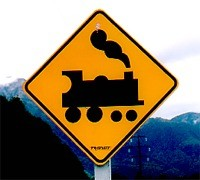
\includegraphics[width=0.2\textwidth]{images/1_seminar_tog_skilt}}

  En jernbaneoverskæring
  \begin{itemize}
  \item Tre komponenter:
    \begin{itemize}
    \item et \textbf{tog}
      \begin{itemize}
      \item krydser vejen
      \item kommunikerer med kontrolsystemet
      \end{itemize}
    \item et \textbf{kontrolsystem}
      \begin{itemize}
      \item styrer bommen
      \end{itemize}
    \item en \textbf{bom}
    \end{itemize}
  \item Sikkerhedsegenskab:
    bommen er altid nede, når toget krydser vejen

  \end{itemize}
\end{frame}

\begin{frame}
  \frametitle{Modellering af systemet}
\begin{tabular}{lll}
Tog & Kontrolsystem & Bom \\
  \includegraphics[width=0.2\textwidth]{images/1_seminar_togmodel_tog} &
  \includegraphics[width=0.2\textwidth]{images/1_seminar_togmodel_kontrol} &
  \includegraphics[width=0.2\textwidth]{images/1_seminar_togmodel_bom}\\
\end{tabular}
  \begin{itemize}
  \item Begivenheder (alfabet):
{\small
\begin{itemize}
\item \textbf{approach}: toget nærmer sig
\item \textbf{cross}:    toget krydser vejen
\item \textbf{exit}:     toget forlader området
\item \textbf{lower}:    besked til bommen om at gå ned
\item \textbf{raise}:    besked til bommen om at gå op
\item \textbf{down}:     bommen går ned
\item \textbf{up}:       bommen går op
\end{itemize}
}
  \end{itemize}
\end{frame}

\begin{frame}
  \frametitle{Modellering som FA}
  Eksempel:
\imagetop{\includegraphics[scale=0.3]{images/1_seminar_togmodel_togFA}}
  \begin{itemize}
\item definer accepttilstande
\item tilføj loop-transitioner så komponenterne får samme alfabet
\item tilføj crash-tilstand og ekstra transitioner \\
  så transitionsfunktionen bliver total
  \end{itemize}
\end{frame}

\begin{frame}
  \frametitle{Kombination af elementerne}
  \begin{itemize}
  \item  Vi er interesseret i de sekvenser af begivenheder,
der opfylder alle komponenterne
\item Produktkonstruktion:
\[L(M) = L(M_{TOG}) ∩ L(M_{KONTROL}) ∩ L(M_{BOM})\]
  \end{itemize}
\end{frame}

\begin{frame}
  \frametitle{Modellering af sikkerhedsegenskaben}
``Bommen er altid nede når toget krydser vejen''


  \begin{itemize}
  \item S:

\begin{center}
{\includegraphics[scale=0.3]{images/1_seminar_togmodel_sikkerhed}}
\end{center}
  \end{itemize}
\end{frame}

\begin{frame}
  \frametitle{Verifikation}
  \begin{itemize}
  \item  Korrekthed: $L(M) ∩ (L(S))’ = ∅$
\item dvs. vi skal bruge
\begin{itemize}
\item produktkonstruktion (igen)
\item komplement
\item algoritme til at afgøre \\ 
  om sproget for en given FA er
\end{itemize}

tomt (3. seminar)
\item hvis $L(M) ∩ (L(S))’ {\color{red}≠} ∅$:
   enhver streng i $L(M) ∩ (L(S))’$ svarer til
   et \textbf{modeksempel} (algoritme: 3. seminar)

  \end{itemize}
\end{frame}

\begin{frame}
  \frametitle{Verifikation med dRegAut-pakken}
  \begin{itemize}
\item Opbyg FA-objekter svarende til
$M_{TOG}, M_{KONTROL}, M_{BOM}$, og $S$
\item Kombiner med \texttt{FA.intersection()} og
\texttt{FA.complement()}
\item Brug \texttt{FA.isEmpty()} og
\texttt{FA.getAShortestExample()}
\item Resultat:

  modeksempel:\\
\ \ \ \textbf{approach · lower · down · up · cross}

  \end{itemize}
\end{frame}

\begin{frame}
  \frametitle{Resume}
  \begin{itemize}[<+->]
  \item Definition af \textbf{endelige automater} og deres sprog
  \item \textbf{Skelnelighed}, hvad repræsenterer tilstandene,
    nødvendigt antal tilstande
  \item \textbf{Produktkonstruktionen}, komplement \emph{(konstruktive beviser)}
  \item \texttt{dRegAut.FA} klassen, Java-repræsentation af FA’er
  \item Eksempel: automater til modellering og verifikation

  \end{itemize}
\end{frame}

\end{document}

